% !TeX root = ../tesi.tex

\iniziocapitoloterzo
\chapter{Progetto e sviluppo di ChatCart}

Racconto lo \emph{stage} come un piccolo progetto a sé stante: il metodo di lavoro, l’analisi, la
progettazione, la realizzazione, le sperimentazioni, la verifica e i risultati.

\section{Metodo di lavoro}

\subsection{Pianificazione e interazione con il \emph{tutor} aziendale}
\label{sec:pianificazione}

Il piano di lavoro assegnava 310 ore indicative a dieci attività, senza distribuirle in un
calendario settimanale. La scelta era coerente con la natura esplorativa del progetto, perché Halue
non
sapeva ancora quale forma avrebbe preso un assistente con interfaccia generativa, e un calendario
dettagliato avrebbe fissato in anticipo decisioni che dipendevano da ciò che avrei scoperto
lavorando. Io e il \emph{tutor} abbiamo quindi tenuto fissi gli obiettivi e stabilito di volta in
volta le attività successive in base allo stato del prototipo. Un procedimento di questo tipo
richiede confronti frequenti, che il piano prevedeva quotidiani e settimanali e che ho adattato al
lavoro prevalentemente da remoto (\tabref{tbl:coordinamento-stage}).

\begin{tabellalunga}{P{0.3}P{0.7}}
	{\textbf{Momento previsto} & \textbf{Svolgimento effettivo}}
	{Le modalità di coordinamento durante lo \emph{stage}.}
	{tbl:coordinamento-stage}
	Allineamento quotidiano con il \emph{team} & Ho partecipato allo \emph{stand-up} mattutino,
	riportando attività concluse, lavoro previsto e impedimenti. \\
	Allineamento quotidiano con il \emph{tutor} & Ho inviato un resoconto scritto di fine giornata
	nel canale Slack dedicato. \\
	Revisione settimanale di un’ora & Io e il \emph{tutor} abbiamo discusso il prototipo, i
	problemi aperti e le attività successive. \\
	Supporto su richiesta & Ho chiesto riunioni aggiuntive quando una scelta bloccava il lavoro;
	in alcuni confronti è intervenuto anche il fondatore. \\
	Presenza in sede & Dopo i primi due giorni in ufficio, sono stato in sede in media un giorno
	a settimana. \\
\end{tabellalunga}

Il lavoro da remoto rendeva il confronto meno immediato che in ufficio, e nelle prime settimane
ponevo le domande al \emph{tutor} troppo tardi, dopo aver dedicato tempo a soluzioni che un
confronto anticipato avrebbe corretto. Ho quindi iniziato a preparare ogni confronto per iscritto,
indicando il risultato atteso, le alternative già provate e le decisioni da prendere insieme. La
forma scritta mi obbligava a definire il problema prima della riunione e lasciava traccia della
decisione presa. Per la sincronizzazione del carrello, per esempio, ho presentato tre possibilità:
specializzare il \emph{widget} per un tema, supportare una famiglia di temi oppure offrire
un’integrazione generica. Da quel confronto è nata la combinazione di adattatori e ripiego
descritta nella \secref{sec:widget}; ciò che ho imparato dalla comunicazione a distanza è oggetto
della \secref{sec:maturazione}.

Il primo passaggio importante è arrivato presto. Nella prima settimana ho studiato l’ecosistema
Shopify e definito il perimetro del progetto; nella seconda ho completato un primo prototipo
funzionante, con cui ho verificato le scelte architetturali concordate con il \emph{tutor}. Alla
fine della terza settimana, dopo circa sette giorni passati a lavorare sul codice, avevo una prima
versione che copriva gli obiettivi obbligatori OB1--OB5. Il \emph{tutor} l’ha valutata
positivamente e, con più di metà dello \emph{stage} ancora da svolgere, abbiamo deciso di dedicare
il tempo restante all’esperienza d’uso e alla sperimentazione, che Halue considerava la parte di
maggior valore del progetto. La prima versione è diventata così una base da mettere alla prova, e
funzionalità e architettura hanno continuato a cambiare fino alle ultime settimane.

Per capire quanto questa decisione abbia modificato la distribuzione del lavoro, ho ripartito a
consuntivo le 304 ore dello \emph{stage} tra le attività del piano, basandomi sulla storia delle
modifiche al codice e sulle date dei documenti di progetto. La \figref{fig:tempi-stage} riporta il
risultato in ore intere e indicative.
% DA CONFERMARE: Edoardo riconosce la ripartizione delle ore almeno per ordine di grandezza?

\begin{figure}[htbp]
	\centering
	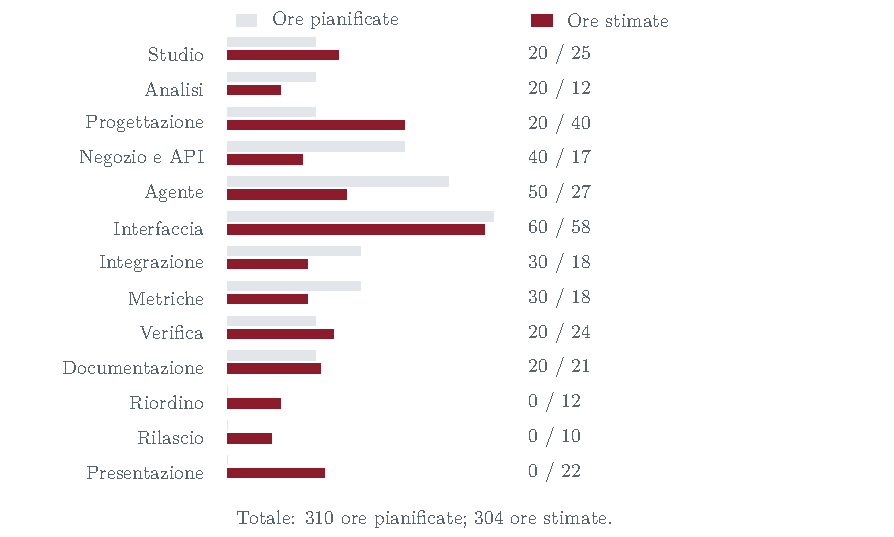
\includegraphics[width=\linewidth]{assets/03-tempi.pdf}
	\caption[Ore pianificate e stimate per attività]{Le ore del piano e la mia stima a consuntivo,
	in valori indicativi. Le ultime tre attività non avevano una voce autonoma nel piano. Le barre
	confrontano quantità di lavoro, senza attribuire al piano un calendario che non prevedeva.}
	\label{fig:tempi-stage}
\end{figure}

La progettazione ha richiesto il doppio delle ore previste, perché vi sono tornato ogni volta che
una prova mostrava un limite della soluzione adottata. La prima realizzazione dell’agente e
dell’accesso al negozio ha richiesto invece circa la metà del tempo previsto, perché il modello
ufficiale di Shopify per le applicazioni forniva già autenticazione, sessioni e integrazione con
l’amministrazione. Lo sviluppo dell’interfaccia si è esteso lungo quasi tutto lo \emph{stage},
comprese le sperimentazioni poi abbandonate, e il tempo risparmiato nelle prime settimane è andato
al riordino del codice, al rilascio e alla presentazione finale al resto del \emph{team}, attività
che il piano non prevedeva come voci autonome. La distribuzione effettiva riflette quindi la
decisione presa alla fine della terza settimana, che ha trasformato un piano pensato per costruire
un prodotto in un percorso di ricerca e sviluppo, in cui provavo ogni soluzione, la valutavo con
il \emph{tutor} e, quando serviva, la rivedevo.

\subsection{Organizzazione del lavoro e tracciamento delle attività}

Illustro come ho organizzato il mio lavoro, svolto in gran parte da remoto: come individuavo le
attività e ne stabilivo le priorità, come ne tenevo traccia e come preparavo le modifiche più estese
prima di realizzarle.

\subsection{Strumenti e assistenti di programmazione}

Presento gli strumenti che ho impiegato per lo sviluppo, la verifica e il rilascio, tra cui gli
assistenti di programmazione basati su modelli linguistici. Di questi descrivo l’uso che ne ho
fatto: la sperimentazione e la validazione rapida delle idee, fino a prototipi funzionanti nell’arco
di una giornata, a cui seguiva l’implementazione definitiva scritta a mano; la stesura dei documenti
di progettazione, per individuare in anticipo i casi limite e i \emph{test} necessari; le attività
di supporto, come la generazione dei dati di prova. Ciò che ho imparato da questo uso lo discuto
nella \secref{sec:maturazione}.

\section{Studio preliminare e analisi}

\subsection{L’ecosistema delle applicazioni Shopify}
\label{sec:ecosistema-applicazioni}

Descrivo la fase iniziale dello \emph{stage}, dedicata allo studio del funzionamento di
un’applicazione Shopify (autenticazione, \emph{app proxy}, estensioni del tema, differenze tra
Storefront API e Admin API) e degli strumenti per la costruzione di agenti. Distinguo le conoscenze
che avevo già acquisito lavorando sui temi Liquid da quelle che ho dovuto costruire per la prima
volta.

\subsection{Un’analisi dei requisiti iterativa}
\label{sec:requisiti}

Motivo la scelta, condivisa con il \emph{tutor}, di non svolgere un’analisi dei requisiti completa
all’inizio del progetto: il lavoro aveva carattere esplorativo, nessun cliente ne dettava i
requisiti, e una specifica fissata a priori sarebbe diventata presto obsoleta. Descrivo il
procedimento che ho seguito: a partire dagli obiettivi del piano ho abbozzato i casi d’uso
principali e ne ho ricavato i requisiti, che ho rivisto a ogni iterazione insieme al prodotto. Un
diagramma mostra i casi d’uso nella loro forma finale e una tabella riporta i requisiti a cui sono
arrivato, raggruppati per area, ciascuno con un identificativo e l’obiettivo del piano da cui
deriva; ne misuro la copertura nella \secref{sec:quantitativi}.

% DA DEFINIRE: prima i casi d'uso iniziali, poi come raggruppare i requisiti (utente, agente, app...). Solo dopo valutare se partire dalla specifica cancellata il 15/10 in chat-cart.

\section{Architettura del sistema}

\subsection{Visione d’insieme}

Illustro l’architettura di ChatCart con un diagramma: il \emph{widget} nel negozio (\emph{app
layer}), il \emph{server} che ospita l’agente (\emph{agent layer}), la \emph{dashboard} del
commerciante e i servizi esterni. Motivo la scelta di uno stile funzionale anziché orientato agli
oggetti, la decisione, su indicazione del \emph{tutor}, di non introdurre astrazioni prima che
fossero necessarie e i \emph{design pattern} che ho adottato quando lo sono diventate.

\subsection{Il contratto tra agente e \emph{widget}}
\label{sec:contratto}

Approfondisco la scelta su cui si regge l’interfaccia generativa: un unico elenco di strumenti,
condiviso tra agente e \emph{widget}, che distingue gli strumenti che leggono i dati del negozio da
quelli che mostrano un componente e chiudono la risposta. Spiego come da questo elenco derivo i tipi
condivisi tra le due parti, così che il \emph{widget} sappia sempre disegnare ciò che l’agente
sceglie.

\section{Realizzazione}

\subsection{L’agente conversazionale}

Descrivo il processo con cui l’agente costruisce una risposta: un ciclo in cui il modello invoca gli
strumenti per consultare il catalogo, finché non seleziona un componente da mostrare. Discuto come
ho ripartito il controllo del comportamento tra le istruzioni al modello e le regole fisse nel
codice, come ho generato i tre messaggi suggeriti e come ho scelto il modello e il livello di
ragionamento, confrontandone velocità e accuratezza. Un diagramma di sequenza segue il percorso di
un messaggio dall’utente alla risposta. Questa parte risponde agli obiettivi OB2 e OB3.

\subsection{Il \emph{widget} e l’integrazione con il tema del negozio}

Presento il \emph{widget}: i componenti (schede prodotto con selezione della variante, schede con le
risposte tratte dalle pagine del negozio, collegamenti alle collezioni), il supporto a più lingue e
valute e, in particolare, la sincronizzazione del carrello con il tema del negozio. Analizzo perché
ogni tema Shopify gestisce il carrello in modo diverso e come ho affrontato il problema con un
\emph{adapter} per ciascun tema e una soluzione di ripiego. Questa parte risponde agli obiettivi
OB1, OB4 e DE1.

\subsection{Metriche di utilizzo e analisi delle conversazioni}

Descrivo gli eventi che il \emph{widget} registra, il \emph{funnel} che la \emph{dashboard} presenta
al commerciante e l’analisi delle conversazioni con Jev, un modello decisionale di TypeSafe AI
uscito durante lo \emph{stage}: a differenza di un modello linguistico generativo, non produce testo
ma restituisce decisioni tipizzate con la loro probabilità. Da qui apro il confronto tra i due tipi
di modello nei compiti decisionali. Questa parte risponde all’obiettivo OB5.

\section{Sperimentazioni e sviluppi futuri}
\label{sec:sperimentazioni}

Dedico questa sezione alle funzionalità che ho sperimentato senza portarle nel prodotto finale,
perché documentano l’orientamento alla ricerca che io e il \emph{tutor} abbiamo dato al progetto
dalla terza settimana: i messaggi di invito che comparivano prima dell’apertura della chat, i tre
tentativi di adattare l’aspetto del \emph{widget} al tema del negozio, l’impiego di Jev nella scelta
dei componenti, il pannello a tutto schermo su \emph{desktop}. Per ciascuna espongo l’ipotesi di
partenza, l’esito che ho osservato e le ragioni per cui io e il \emph{tutor} abbiamo deciso di non
inserirla nel prodotto consegnato. Da queste prove ricavo infine le strade lungo cui ChatCart
potrebbe evolvere in futuro.

% DA CONFERMARE: quali strade di evoluzione indicare.

\section{Verifica e validazione}
\label{sec:verifica}

Illustro la mia strategia di verifica: \emph{test} automatici concentrati sui punti in cui ChatCart
interagisce con sistemi esterni che non controllo, eseguiti su una base di dati reale e senza
simulare i moduli interni, e le ragioni di questa scelta. Discuto i limiti dei \emph{test}
tradizionali applicati a un agente che non risponde mai due volte nello stesso modo. Concludo con la
validazione svolta insieme al \emph{tutor} e con il rilascio dell’applicazione \emph{online}.

\section{Risultati}

\subsection{Il prodotto dal punto di vista dell’utente}

Presento ChatCart dal punto di vista di chi lo utilizza, attraverso una sequenza di schermate: un
cliente che cerca un prodotto, lo confronta con altri, lo aggiunge al carrello e raggiunge il
pagamento; poi il commerciante che consulta il \emph{funnel} e le conversazioni nella
\emph{dashboard}. Dichiaro inoltre i limiti noti del prototipo.

\subsection{Risultati quantitativi}
\label{sec:quantitativi}

Riporto in tabelle i dati quantitativi del progetto: la copertura dei requisiti definiti nella
\secref{sec:requisiti}, la copertura dei \emph{test} con le scelte che la motivano, le righe di
codice per ciascuna parte dell’applicazione e i documenti che ho consegnato al \emph{team}.

\finecapitoloterzo
